\documentclass{beamer}
\usetheme{Madrid} % Required for inserting images
\usefonttheme{professionalfonts}
\usepackage{tabularx}
\title{Evaluation of Cryptographic Protocols for Secure
Communication in Artificial Pancreas Systems}
\author{Suhasini Prakash}
\institute{Institute for Computing in Research}
\date{July 2026}

\begin{document}
\begin{frame}[plain] 
    \titlepage
\end{frame}


\begin{frame}{Motivation}
    \begin{itemize}
        \item Estimated 2.5 million users of artificial pancreas systems
        \item Secure communication needed to prevent tampering of data/insulin commands
        \item Limited computational power of systems make heavy security protocols difficult to implement
    \end{itemize}
    
\end{frame}

\begin{frame}{High Level Architecture}
    \begin{figure}
        \centering
        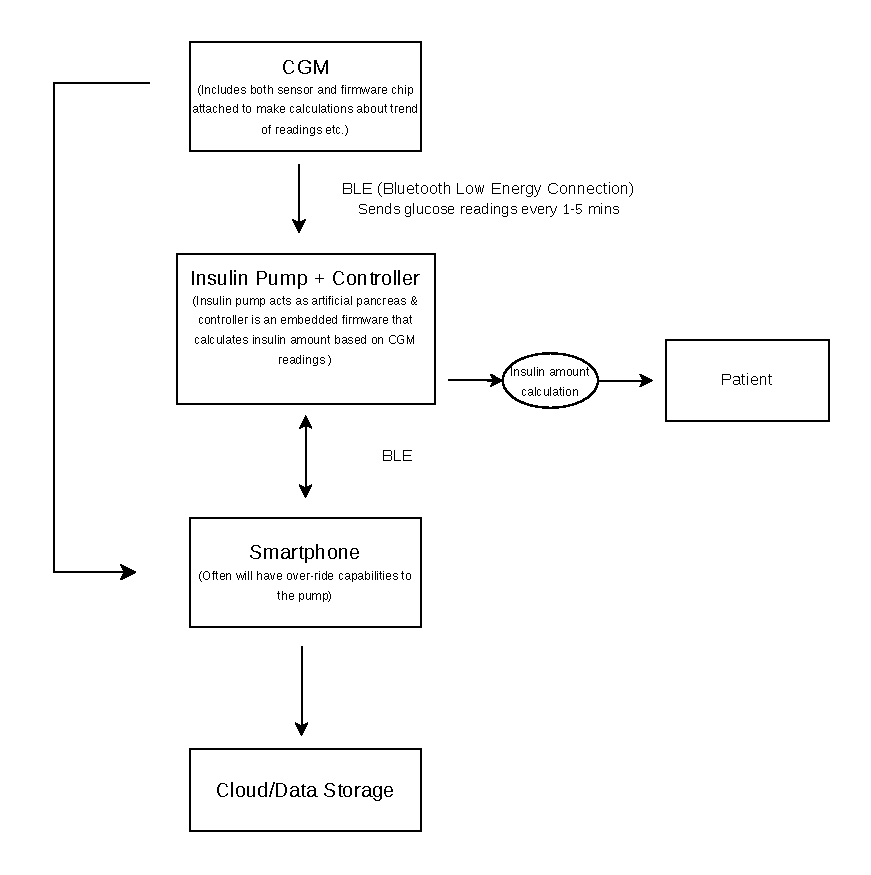
\includegraphics[width=0.65\linewidth]{HighLevelArchitecture.pdf}
 
    \end{figure}
\end{frame}
\begin{frame}{STPA-Sec}
    Why STPA-Sec?
    
    \begin{itemize}
        \item Analyze communication subsystem /& losses associated with communication failure
        \item Safety-informed evaluation criteria for STPA-Sec
    \end{itemize}
\end{frame}
\begin{frame}{STPA-Sec Analysis - Control Structure}
    \begin{figure}[H]
    \centering
    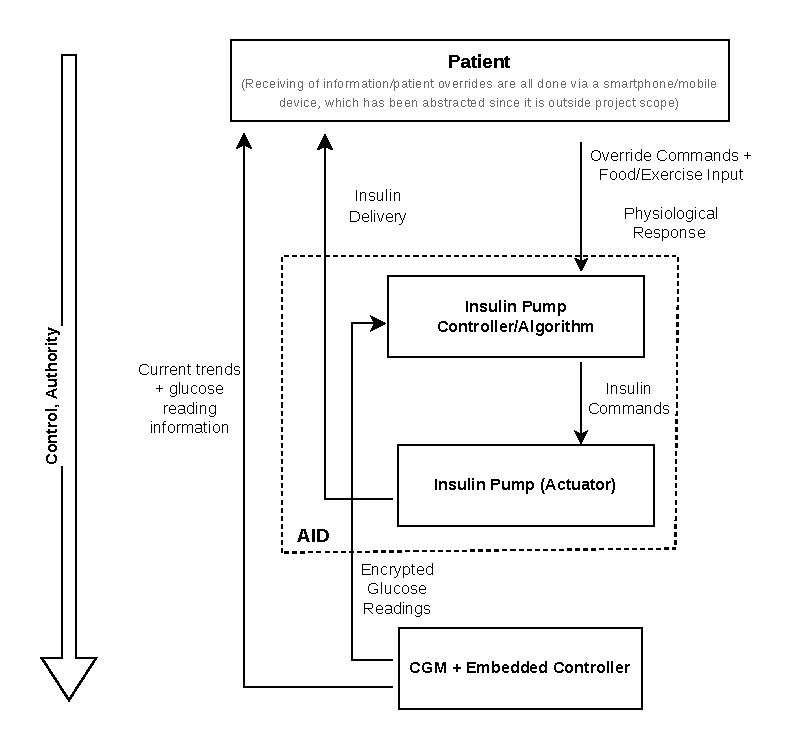
\includegraphics[width=0.5\linewidth]{STPAControlStructure.pdf}
    \caption{Hierarchical STPA Control Structure}
    \label{fig:placeholder}
\end{figure}
\end{frame}
\begin{frame}{STPA-Sec Analysis - Unsafe Control Actions}
    
\end{frame}
\begin{frame}{Scope}
    Inside Scope
    \begin{itemize}
        \item CGM /& AID communication
        \item  Symmetric encryption protocols for messages/glucose readings
        \item Computational overhead for encryption algorithms
        \item Security requirements derived from STRIDE /& STPA Sec frameworks
    \end{itemize}
\end{frame}
\begin{frame}{Scope}
    
    Outside Scope
    \begin{itemize}
        \item BLE connection reliability
        \item Connection to smartphone/mobile devices
        \item Data storage in cloud/hospital system
    \end{itemize}
\end{frame}

\begin{frame}{Assumptions}
        \begin{itemize}
            \item Simulation is conducted on computer hardware rather than embedded hardware of artificial pancreas system - results are a relative comparison
            \item All encryption algorithms are implemented correctly in Python libraries
        \end{itemize}
\end{frame}

\begin{frame}{Simulation Overview}
    \begin{itemize}
        \item Communication between CGM and insulin pump
        \item Communication channel simulated using Python program
        \item One time asymmetric key exchange via ECDH
    \end{itemize}
\end{frame}


\begin{frame}{Encryption Algorithm Comparison}
    \begin{table}[htbp]
    \caption{Symmetric Encryption Algorithms}
    \begin{center}
    \begin{tabularx}{\textwidth}{|X|X|X|}
    \hline
    \textbf{Algorithm} & \textbf{Represents} & \textbf{Expected Tradeoff} \\
    \hline
    \texttt{AES-CBC} & \texttt{Confidentiality Only} & \texttt{No integrity, low overhead} \\
    \hline
    \texttt{AES-CBC + HMAC} & \texttt{Legacy Authenticated Encryption} & \texttt{High overhead, improved security} \\
    \hline
    \texttt{AES-CCM} & \texttt{BLE Standard} & \texttt{Secure + Efficient} \\
    \hline
    \texttt{AES-GCM} & \texttt{Modern AES} & \texttt{Modern-day Baseline} \\
    \hline
    \texttt{ChaCha20Poly1305} & \texttt{Software-optimized Modern Protocol} & \texttt{Most Software-Efficient} \\
    \hline
    \end{tabularx}
    %\label{tab1}
    \end{center}
\end{table}

\end{frame}

\begin{frame}{Simulation Results - Memory Benchmarking}
    \begin{figure}
        \centering
        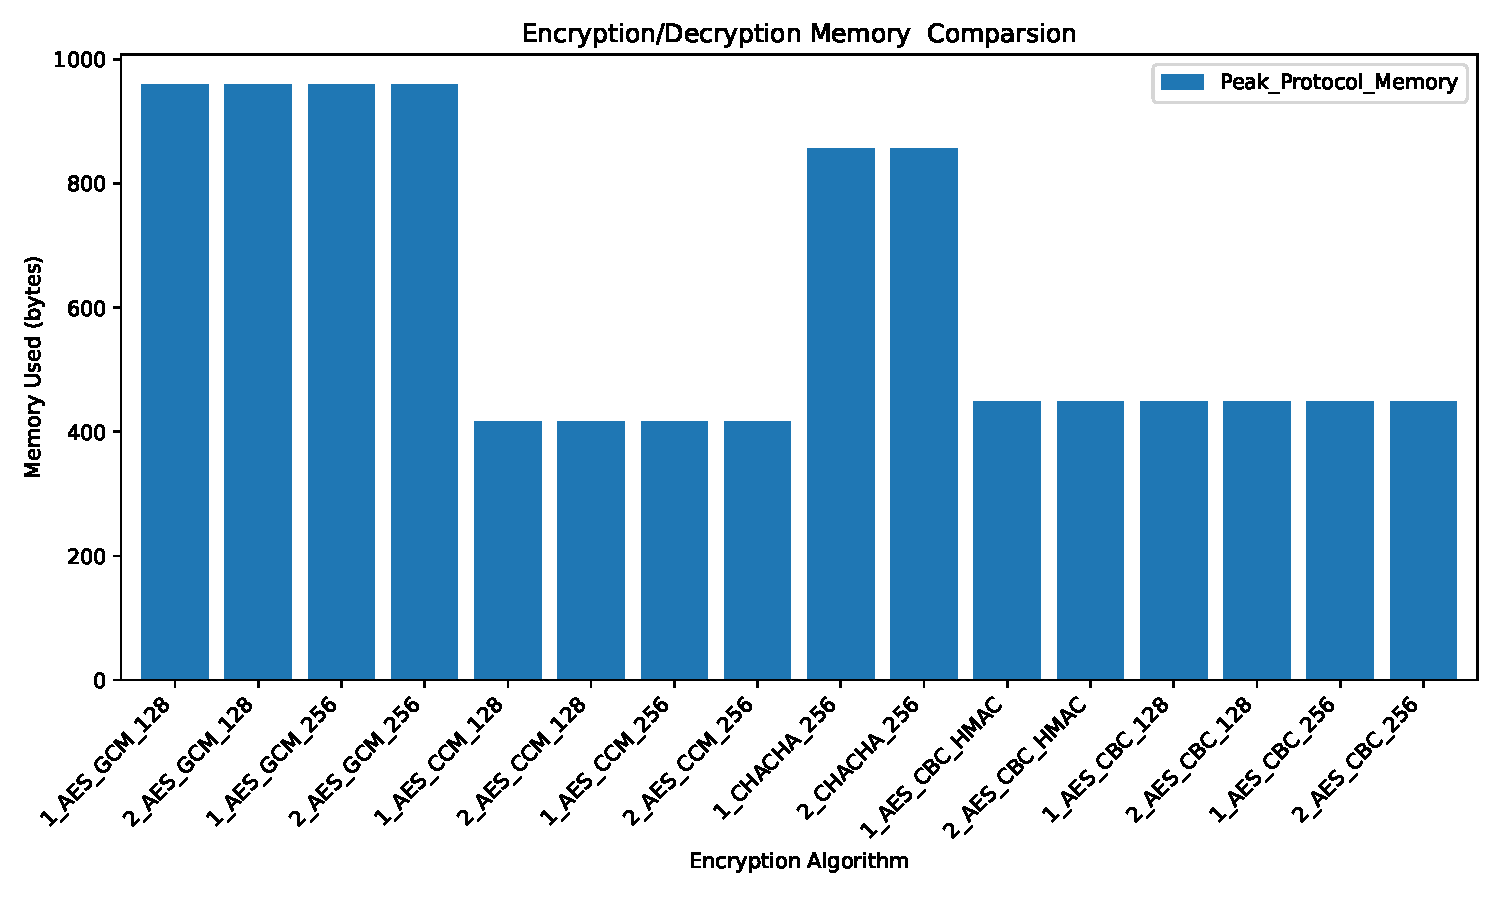
\includegraphics[width=0.9\linewidth]{MemoryBenchmark.pdf}
        
    \end{figure}
\end{frame}

\begin{frame}{Simulation Results - Time Benchmarking}
    
    \begin{figure}
        \centering
        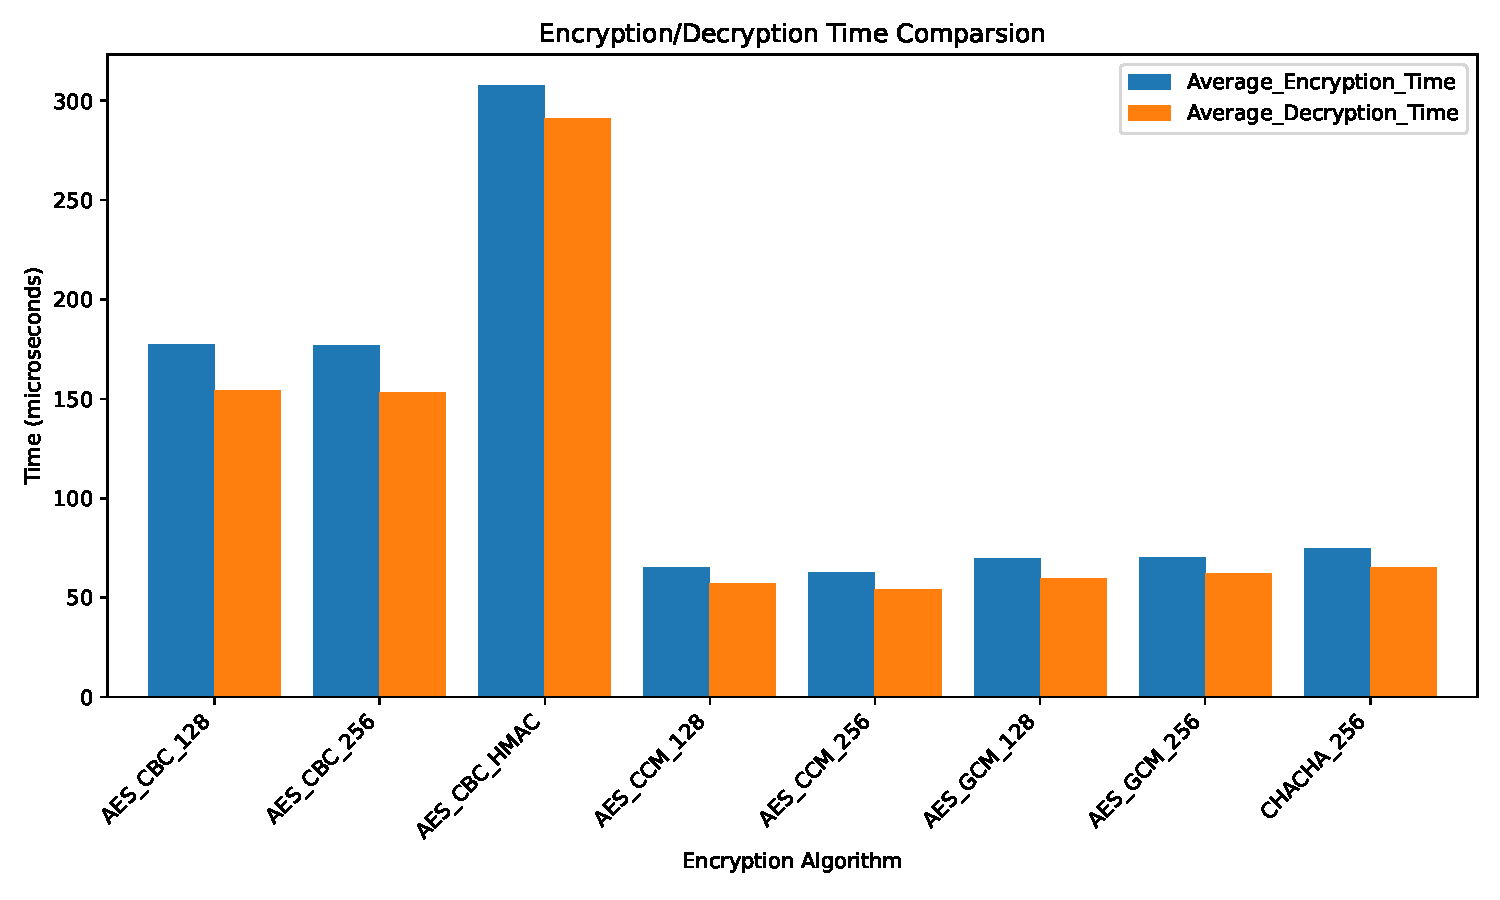
\includegraphics[width=0.9\linewidth]{TimeBenchmark.pdf}
    \end{figure}
\end{frame}

\begin{frame}{Discussion}
    Key Takeaways         
    \begin{itemize}
        \item Modern AEAD protocols provided best security + limited overhead
        \item Limited computational differences between CCM \& GCM \& ChaCha - Should use security to drive choices
    \end{itemize}
\end{frame}

\begin{frame}{Limitations \& Future Work}
    \begin{itemize}
        \item Results should be modeled on CGM/AID hardware
        \item Extend simulation to include comparison of initial key exchange/asymmetric encryption protocols 
    \end{itemize}
\end{frame}

\begin{frame}{Thank You}
    \begin{center}
        Questions?
    \end{center}
\end{frame}
\begin{frame}{Appendix - STRIDE Threat Model}
    \begin{center}
        \begin{figure}
        \centering
        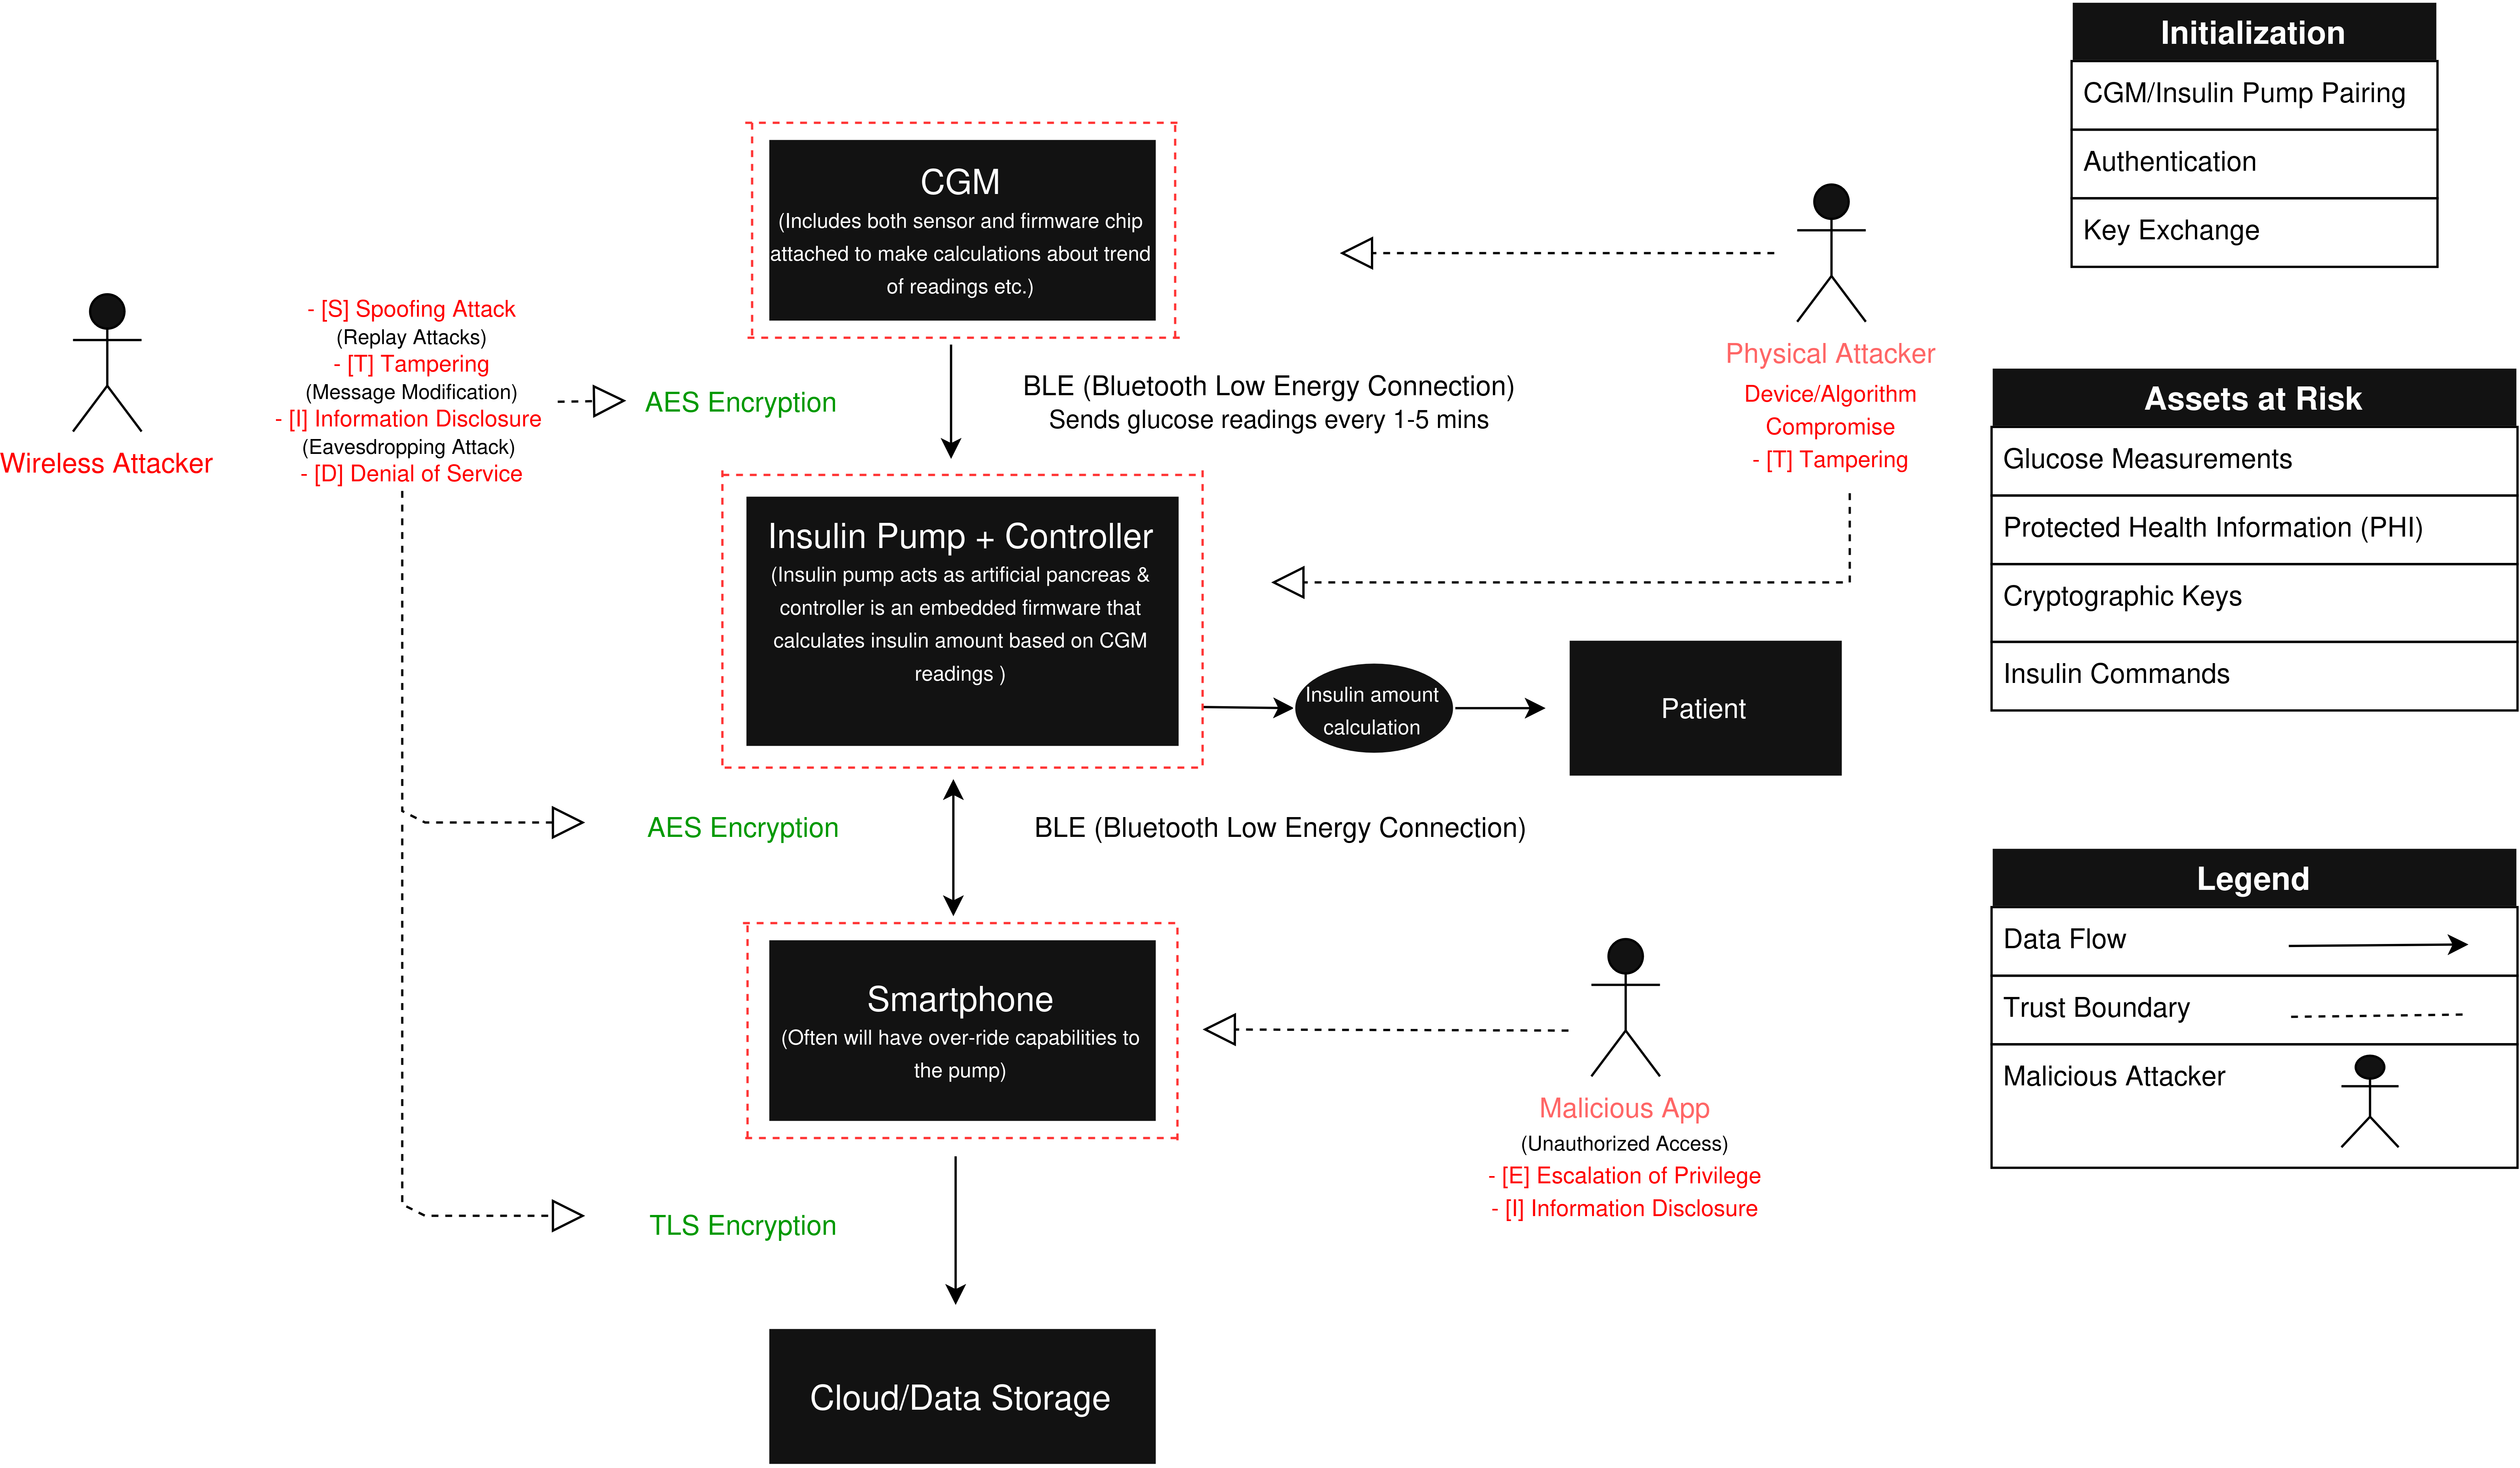
\includegraphics[width=0.9\linewidth]{STRIDEThreatModel.png}
        \end{figure}
    \end{center}
\end{frame}
\end{document}
